% 
% Septiembre 2020
% Author: Mathieu Kessler
% Universidad Politécnica de Cartagena
% https://personas.upct.es/perfil/mathieu.kessler
% 
% 
\documentclass[9pt]{beamer}
\definecolor{links}{HTML}{2A1B81}
\hypersetup{colorlinks,linkcolor=,urlcolor=links}
 \usepackage[spanish]{babel}
\usepackage{colortbl}
\usepackage{graphicx}
\usepackage{amsmath,amssymb}
\usepackage{comma}
\usepackage{fancybox,color}
\usepackage[utf8]{inputenc}
\graphicspath{{../figures/}}
\setbeamertemplate{navigation symbols}{}
% -----------------------------------------------------------------------------
% To include multple images sequentially
% https://codeyarns.com/2010/02/09/how-to-do-image-animation-in-beamer/
% ------------------------------------------------------------------------------
 \usepackage{xmpmulti}
%------------------------------------------------------------------------------
\usepackage{xcolor}
\definecolor{mycodecolor}{rgb}{0.65,0.25,0.1}
\newcommand{\inlinecode}[1]{{\tt \textcolor{mycodecolor}{#1}}}
\usepackage{pythontex}
%--------------------
\usepackage{beamerthemeshadow}
\usepackage{xmpmulti}
\usepackage{mathtools}
\DeclarePairedDelimiter\abs{\lvert}{\rvert}%
\usepackage{tabularx}
\renewcommand\tabularxcolumn[1]{b{#1}}
\newcommand{\field}[1]{\mathbb{#1}}
\newcommand{\E}{\field{E}}
\newcommand{\R}{\field{R}}
\newcommand{\N}{\field{N}}
\newcommand{\Z}{\field{Z}}
\newcommand{\Q}{\field{Q}}
\newcommand{\EE}{\field{E}}
\newcommand{\FF}{\field{F}}
\newcommand{\GG}{\field{G}}
\renewcommand{\L}{\field{L}}
\renewcommand{\P}{\field{P}}
\newcommand{\LL}{{\mathfrak L}}

% define el folder donde del workspace, para cambiar inglés, ids,
% etc..
\newcommand{\workspacefolder}{stat\_labs }


\begin{document}
\title{Pandas: cómo acceder a columnas o filas de un DataFrame, seleccionar subconjuntos}

\author[Mathieu Kessler]{Mathieu Kessler}
\institute[]{Departamento de Matemática Aplicada y Estadística \\ Universidad Politécnica de Cartagena}
\date{@kessler\_mathieu}{}%{\href{https://code.visualstudio.com}{https://code.visualstudio.com}}
\titlegraphic{
\includegraphics[width=3cm]{1200px-Pandas_logo.svg.png}}

\begin{frame}
  \titlepage
\end{frame}

\begin{frame}[fragile]
  \frametitle{Las operaciones más frecuentes implican trabajar con subconjuntos}
  \begin{block}{}
Esos subconjuntos de un DataFrame pueden ser de diferentes tipos:
    \begin{itemize}
    \item {\footnotesize Extraigo un conjunto de columnas relevantes, descartando otras.}
      \begin{center}
        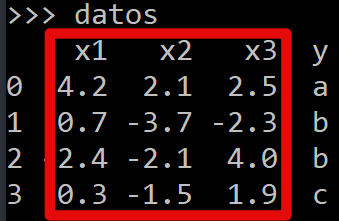
\includegraphics[width=2.5cm]{seleccionar_columnas}
      \end{center}
    \item {\footnotesize Me quedo con un subconjunto de filas que cumplen un determinado criterio}
      \begin{center}
        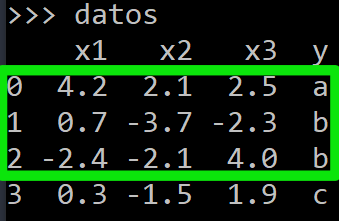
\includegraphics[width=2.5cm]{seleccionar_filas}
      \end{center}
    \item {\footnotesize Una combinación de las dos opciones anteriores}
      \begin{center}
        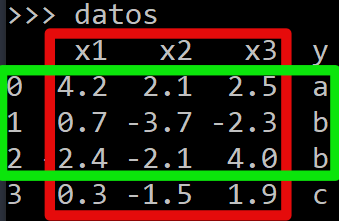
\includegraphics[width=2.5cm]{seleccionar_columnas_filas}
      \end{center}
    \end{itemize}
  \end{block}
    \end{frame}
\begin{frame}[fragile]
  \frametitle{Extraer columnas}
  \begin{block}{Para extraer un conjunto de columnas relevantes}
    La manera más sencilla es indicar  entre llaves una etiqueta o una lista de las etiquetas de columnas que deseo extraer
  \end{block}
  \begin{pyconcode}
import pandas as pd
import numpy as np
rng = np.random.default_rng(314)
x = np.round(rng.uniform(-5, 5, (4, 3)), 1)
#datos = pd.DataFrame({'x1': [2.1, 3, -0.5, 1.8],
#  'x2': [-0.4, 0, 3.1, -1],
#  'x3': [-2, 0.8, 2.4, 3.5],
#  'y': ['a', 'b', 'b', 'c']})
datos = pd.DataFrame(
    x,
    columns=['x1', 'x2', 'x3']
    )
datos['y'] = ['a', 'b', 'b', 'c']
datos2 = datos.copy()
  \end{pyconcode}
\pause
\begin{itemize}
  \item<2-> Para seleccionar solamente una columna:
    \begin{pyconsole}
datos['x2']
    \end{pyconsole}
    \onslide<4->{\begin{center}
        \alert{NOTA: el resultado es un Series}
         \end{center}}
  \item<3-> Para seleccionar varias columnas
        \begin{pyconsole}
datos[['x1', 'x2']]
        \end{pyconsole}
            \onslide<5->{\begin{center}
                \alert{NOTA: el resultado es un DataFrame}
            \end{center}}
\end{itemize}
\end{frame}
\begin{frame}[fragile]
  \frametitle{Extraer filas basándose en un criterio}
  \begin{block}{Para seleccionar filas basándose en un criterio lógico}
    La manera más sencilla es indicar entre llaves un objeto de tipo vector (lista, array numpy, Series)  booleano (True o False)
  \end{block}
\pause
\begin{itemize}
  \item<2-> Por ejemplo:
    \begin{pyconsole}
datos[[False, True, True, False]]
    \end{pyconsole}
  \item<3-> Podemos proporcionar un Series calculado
        \begin{pyconsole}
datos[datos['y'] == 'b']
        \end{pyconsole}
\end{itemize}
            \onslide<4->{\begin{center}
                \alert{NOTA: se preservan las etiquetas (index) de las filas}
            \end{center}}
\end{frame}
\begin{frame}[fragile]
  \frametitle{La manera más general de seleccionar filas y/o columnas}
  \begin{block}{Los dos métodos  más flexibles y generales para seleccionar filas y/o columnas}
    \begin{itemize}
    \item
      El método {\tt loc} permite seleccionar filas y/o columnas a través de las etiquetas (index o nombres de columnas) o usando vectores booleanos
    \item El método {\tt iloc} permite seleccionar filas y/o columnas a través de sus posiciones (filas o columnas) o usando vectores booleanos
    \end{itemize}
  \end{block}

\end{frame}
\begin{frame}[fragile]
  
  \begin{block}{El método {\tt loc[]}}
    Se aplica con llaves, separamos la especificación de filas y columnas por una coma. {\tt df.loc[especificacion\_filas, especificacion\_columnas]}
  \end{block}

  \pause
  Recordad el DataFrame {\tt datos}:\smallskip

  \pycon{datos}
  
\begin{itemize}
  \item<3-> Si no hay especificación para filas, usamos ``:'' para indicar que las seleccionamos todas:
    \begin{pyconsole}
datos.loc[:, ['x1', 'x2', 'x3']]
    \end{pyconsole}
\end{itemize}
\end{frame}
\begin{frame}[fragile]
  \frametitle{El método {\tt loc[]}}
 
\begin{itemize}
\item Podemos usar un vector booleano, tanto para filas como para columnas.
      \begin{pyconsole}
datos.loc[:, [True, True, True, False]]
      \end{pyconsole}
    \item<2-> O combinar vectores booleanos con especificación de etiquetas
      \begin{pyconsole}
datos.loc[datos['y'] == 'b', ['x1', 'x2', 'x3']]
      \end{pyconsole}
\end{itemize}
\end{frame}

\begin{frame}[fragile]
  
  \begin{block}{El método {\tt iloc[]}}
    Se aplica con llaves, separamos la especificación de filas y columnas por una coma. Utilizamos sus posiciones para seleccionar filas o columnas. No admite vectores  booleanos.
  \end{block}

  \pause
  Recordad el DataFrame {\tt datos}:\smallskip

  \pycon{datos}
  
\begin{itemize}
  \item<3-> 
    \begin{pyconsole}
datos.iloc[:, [0, 1, 2]]
    \end{pyconsole}
  \item<4->
    \begin{pyconsole}
datos.iloc[[1, 2], [0, 1, 2]]
    \end{pyconsole}
\end{itemize}
\end{frame}

 \begin{pyconcode}
datos_2 = datos.loc[::-1,:]
  \end{pyconcode}
\begin{frame}[fragile]
  \frametitle{El método {\tt loc[]}}
  El método {\tt loc} trabaja con etiquetas, por lo que es necesario ser cautos si el index de nuestro DataFrame son los enteros. Considerad el DataFrame {\tt datos\_2}:\smallskip

  \pycon{datos_2}
  \begin{itemize}
  \item<2->
  \pyv{datos_2.loc[0, :]} no nos devuelve la primera fila (posición 0) sino la cuarta, que es la que tiene etiqueta ``0''.

    \begin{pyconsole}
datos_2.loc[0,:]
    \end{pyconsole}
  \item<3-> 
    \pyv{datos_2.iloc[0,:]} sí nos devuelve la primera fila:

    \begin{pyconsole}
datos_2.iloc[0,:]
    \end{pyconsole}
  \end{itemize}
\end{frame}
\begin{pyconcode}
datos.index = ['a1', 'a2', 'a3', 'a4']
import numpy as np
\end{pyconcode}

\begin{frame}[fragile]
  \frametitle{Cortes (slices) en DataFrames}
  \begin{block}{}
    Al igual que para listas, es posible especificar cortes (slices) en DataFrames o Series, usando ``:''. El corte incluye las columnas o filas comprendidas entre los dos extremos de la especificación. 
  \end{block}\pause
  Considerad el DataFrame datos donde hemos añadido un índice:\smallskip
  
{\footnotesize
  \pycon{datos}
  }
 
  \begin{itemize}
  \item<3-> Para {\tt loc}, usamos especificación por etiquetas:
    \begin{pyconsole}
datos.loc['a2':'a4', :]
    \end{pyconsole}
  \item<4-> Para {\tt iloc}, usamos posiciones
    \begin{pyconsole}
datos.iloc[1:2, 0:2]
    \end{pyconsole}
  \end{itemize}
  \onslide<5->{
  \begin{block}{}
    Para {\tt loc} los dos extremos están incluidos, para {\tt iloc} no está incluido el extremo de la derecha.
  \end{block}}
\end{frame}
\begin{frame}[fragile]
  \frametitle{Cambiar valores en subconjuntos de un DataFrame}
  \begin{block}{}
    Usando {\tt loc} o {\tt iloc} es posible cambiar los valores en un subconjunto del DataFrame.
  \end{block}
 \pause
  Considerad el DataFrame datos:\smallskip
  
{\footnotesize
  \pycon{datos2}
  }
\pause

Podemos fijar el subconjunto a un único valor:
   \begin{pyconsole}
datos.loc[['a2', 'a4'], 'y'] = np.NaN
datos
    \end{pyconsole}
\end{frame}
\begin{frame}[fragile]
  \frametitle{Cambiar valores en subconjuntos de un DataFrame}
  \begin{block}{}
    También podemos asignar a un subconjunto un objeto de tipo vector (lista, numpy array, Series o DataFrame) de dimensiones compatibles con el subconjunto.
  \end{block}
Recordad  el DataFrame datos:\smallskip
  
{\footnotesize
  \pycon{datos2}
  }
\pause



   \begin{pyconsole}
datos.loc[['a2', 'a4'], 'y'] = ['YES', 'NO']
datos
    \end{pyconsole}
\end{frame}
\begin{frame}[fragile]
  \frametitle{Cambiar valores en subconjuntos de un DataFrame}
  \begin{block}{}
    Si usamos un Series o DataFrame, los índices deben coincidir
  \end{block}
Recordad  el DataFrame datos:\smallskip
  
{\footnotesize
  \pycon{datos2}
  }
\pause

{\footnotesize
   \begin{pyconsole}
datos.loc[['a2', 'a4'], 'y'] = pd.Series(['YES', 'NO']) 
datos
   \end{pyconsole}
   \pause
   \alert{El Series de la derecha tiene los índices por defecto (0, 1) que no están en el DataFrame de la derecha}
\pause
      \begin{pyconsole}
datos.loc[['a2', 'a4'], 'y'] = pd.Series(['Y', 'N'], index=['a2', 'a4']) 
datos
   \end{pyconsole}
}
   
\end{frame}
  \begin{pyconcode}
import pandas as pd
import numpy as np
rng = np.random.default_rng(314)
x = np.round(rng.uniform(-5, 5, (4, 3)), 1)
#datos = pd.DataFrame({'x1': [2.1, 3, -0.5, 1.8],
#  'x2': [-0.4, 0, 3.1, -1],
#  'x3': [-2, 0.8, 2.4, 3.5],
#  'y': ['a', 'b', 'b', 'c']})
datos = pd.DataFrame(
    x,
    columns=['x1', 'x2', 'x3']
    )
datos['y'] = ['a', 'b', 'b', 'c']
datos.index = ['a1', 'a2', 'a3', 'a4']
  \end{pyconcode}
\begin{frame}[fragile]
  \frametitle{Cambiar valores en subconjuntos de un DataFrame}
  A veces se usa indexación en cadena en lugar de usar {\tt loc}:
Recordad  el DataFrame datos:\smallskip
  
{\footnotesize
  \pycon{datos}
  }
\pause

\begin{pyconsole}
datos[~(datos['y'] == 'b')]['y']
\end{pyconsole}
\pause
devuelve el mismo objeto que
\begin{pyconsole}
datos.loc[~(datos['y'] == 'b'), 'y']
\end{pyconsole}

\pause
\begin{block}{ AVISO}
  Sin embargo, NO se debe usar la primera forma para asignarle un valor
  \begin{pyverbatim}
datos[~(datos['y'] == 'b')]['y'] = 'b'
  \end{pyverbatim}
  Es de mucho preferible usar {\tt loc} para ello
\begin{pyverbatim}
datos.loc[~(datos['y'] == 'b'), 'y'] = 'b'
\end{pyverbatim}
  \end{block}

   
\end{frame}
\end{document}
